\section{Indocyanine Green}
Due to the difficultly in isolating single-chirality solutions of CNTs, as outlined in in the previous chapter, indocyanine green (ICG) - a fluorescent dye often used in microscopy imaging\cite{farrakhova, spartalis} - was initially used in place of CNTs in the fiber.  This particular dye is an organic semiconductor with Homo-Lumo gap calculations estimating a $~2$eV energy gap, with variations depending on the solvent\cite{Fang}. The HOMO and LUMO energy levels in organic semiconductors are parallel to the maximum valence and minimum conduction, and the aforementioned energy gap falls within the range of energy bandgaps found in inorganic semiconductors. 
\begin{figure}[h]
	\centering
	\foreach \x in {Homo_Lumo, chemical_formula}
	{ 
		\begin{subfigure}[b]{0.45\textwidth}
			\includegraphics[width=\textwidth]{./Figures/ICG/\x.png}
			\caption{}
		\end{subfigure}
		\hfil
	}
	\caption{(a) Depiction of the Homo-Lumo gap in organic semiconductors and the transition occurring between ground and excited states. (b) The chemical structure of ICG provided by MP Biomedicals. }
	\label{fig:homolumo}
\end{figure}
\clearpage
The following section details the the optical properties of ICG and measurements of the optical properties when confined in HCPCF. 

\subsubsection{ Absorption Cross-Section}
ICG absorbs wavelengths between 600-900nm. The absorption is largely bimodal, with the greatest excitation occurring at 780nm and 700nm, but transforms into a monomeric distribution at 780nm at low concentrations and 700nm at high concentrations. 
\begin{figure}[h]
	\centering
	\foreach \x in {D2O_acs, H2O_acs}
	{ 
		\begin{subfigure}[b]{0.49\textwidth}
			\includegraphics[width=\textwidth]{./Figures/ICG/\x.png}
			\caption{}
		\end{subfigure}
		\hfil
	}
	\caption{ Absorption cross-section at peak wavelengths 700nm(blue) and 780nm(green) for ICG dissolved in D2O(a) and H2O(b) .  Data from (cite) was fitted using a linear regression model. }
	\label{fig:icg abs plots}
\end{figure}
Due to the chemical formation of ICG, the absorption of the molecule when dissolved in a solvent is highly concentration-dependent. ICG is made up of monomers, which are a type of molecule that can react with other monomers to form polymer chains. In the case of ICG, its monomers react with each other to form dimers, a chain of two join monomers. With higher concentrations, monomers are closer in proximity and the molecules are more likely shift from monomers to dimers which are less likely to be excited and shift the center absorption wavelength. The concentration of monomer $M$ to dimmers $D$ is governed by the equilibrium reaction
\begin{equation}
	M+M\rightleftarrows D
\end{equation}
and law of mass action relation concentration 
\begin{equation}
	[D] =  K_D[M]^2
\end{equation}
Where $K_D$ is the dimmerization constant . Written in terms of concentration $C$ and mole fractions, $[M] = x_MC= (1-x_D)C $ and $[D]=\frac{x_D}{2}C$., the  mole fraction of dimmers can be written in terms of the dimmerization constant and concentration.
\begin{equation}
	x_D = 1 + \frac{1}{4K_DC} - \sqrt{\big( 1 + \frac{1}{4K_DC}\big)^2-1}
	\label{xd}
\end{equation}
 The absorption cross-section model for ICG\cite{mauerer, philip} will be an average of the affects of the of monomers and dimmers, where d $\sigma_M$ and $\sigma_D$ are the monomer and dimer absorption cross-sections respectively.
\begin{equation}
	\sigma = x_M \sigma_M + x_D \sigma_D = \sigma_M - x_D(\sigma_M - \sigma_D)
	\label{abc}
\end{equation}
Plugging (\ref{xd}) into (\ref{abc}), remaining parameters could be found by doing a linear regression fit to absorption cross-section vs. concentration data from literature and the expected absorption cross-section could be calculated for any concentration. For ICG dissolved in H2O, the existing literature has some variation and so the upper/lower bounds and average were taken, while little data was available for ICG dissolved in D2O. The behavior in H2O and D2O are quite similar and are plotted in Fig\ref{fig:icg abs plots}. At lower concentrations the absorption cross-section is slightly greater for D2O than H2O, with the reverse for high concentrations. 
\clearpage
\begin{table}
	\centering
	\begin{tabularx}{0.8\textwidth} { 
		| >{\centering\arraybackslash}X 
		| >{\centering\arraybackslash}X 
		| >{\centering\arraybackslash}X 
		| >{\centering\arraybackslash}X | }
		\hline
		$\lambda_{peak} = 780nm$ & $K_D$ & $\sigma_M$ & $\sigma_D$\\
		\hline
		\cite{holzer} & $6.01x10^5$ & $9.29x10^{-16}$ & $2.28x10^{-16}$\\
		\hline
		\cite{landsman} & $1.03x10^5$ & $6.74x10^{-16}$ & $1.54x10^{-16}$\\
		\hline
		\cite{mauerer} & $1.40x10^5$ & $6.72x10^{-16}$ & $1.11x10^{-16}$\\
		\hline
		Average & $3.06x10^6$ & $7.94x10^{-16}$ & $1.72x10^{-16}$\\
		\hline
	\end{tabularx}
	\captionof{table}{Absorption Cross Section parameter fitting of ICG  dissolved in deionized water. Fitting done with linear regression on $\sigma$ vs. concentration data measured at $\lambda=780nm$ from  literature. \label{h2o780}}
\end{table}
\begin{table}
	\centering
	\begin{tabularx}{0.8\textwidth} { 
		| >{\centering\arraybackslash}X 
		| >{\centering\arraybackslash}X 
		| >{\centering\arraybackslash}X 
		| >{\centering\arraybackslash}X | }
		\hline
		$\lambda_{peak} = 700nm$ & $K_D$ & $\sigma_M$ & $\sigma_D$\\
		\hline
		\cite{holzer} & $3.00x10^3$ & $2.29x10^{-16}$ & $25.68x10^{-16}$\\
		\hline
		\cite{mauerer} & $3.06x10^4$ & $8.89x10^{-16}$ & $3.93x10^{-16}$\\
		\hline
		Average & $9.31x10^3$ & $1.62x10^{-16}$ & $4.74x10^{-16}$\\
		\hline
	\end{tabularx}
	\captionof{table}{Absorption Cross Section parameter fitting of ICG  dissolved in deionized water. Fitting done with linear regression on $\sigma$ vs. concentration data at $\lambda=700nm$ from literature. \label{h2o700}}
\end{table}	
\begin{table}
	\centering
	\begin{tabularx}{0.8\textwidth} { 
		| >{\centering\arraybackslash}X 
		| >{\centering\arraybackslash}X 
		| >{\centering\arraybackslash}X 
		| >{\centering\arraybackslash}X | }
		\hline
		$\lambda_{peak}$ & $K_D$ & $\sigma_M$ & $\sigma_D$\\
		\hline
		$780nm$ & $3.22x10^4$ & $7.14x10^{-16}$ & $2.68x10^{-17}$\\
		\hline
		$700nm$ & $1.67x10^4$ & $2.833x10^{-16}$ & $6.28x10^{-16}$\\
		\hline
	\end{tabularx}
	\captionof{table}{Absorption Cross Section parameter fitting of ICG  dissolved in heavy water. Fitting done with linear regression on $\sigma$ vs. concentration data at $\lambda=700nm$ from literature. \label{d20700780}}
\end{table}
\clearpage

\subsubsection{ Photostability}
At high concentrations, ICG behaves as a  "J-aggregate", a category of dyes that have a shift in absorption band to larger wavelengths in certain solvents. When mixed into water and other solvents, ICG shifts over time to a center wavelength of 893nm. This process can be accelerated under high heat in high-concentration (in the range of 1000ppm solutions) forms \cite{rotermund},  J-aggregates can be stored at room temperature for several months. However, at such a state the dye will be too optically dense to observe any optical excitation and when diluted to perform such measurements, the J-aggregates will begin to detach into smaller molecules within 24hrs.  The effects of dye concentration of storage life in aqueous solutions becomes a tricky balance at single-digit ppm concentrations, where the fluorescence intensity of the dye is at its greatest but with degradation to undetectable levels occurring in a couple of hours at best if in optimal storage conditions\cite{landsman, saxena}. The rate of deterioration occurs so linearly based on the initial concentration of ICG\cite{holzer}, but the amount of light exposure of the solution will also exasperate the degradation rate\cite{saxena}. 
\begin{figure}[h]
	\centering
	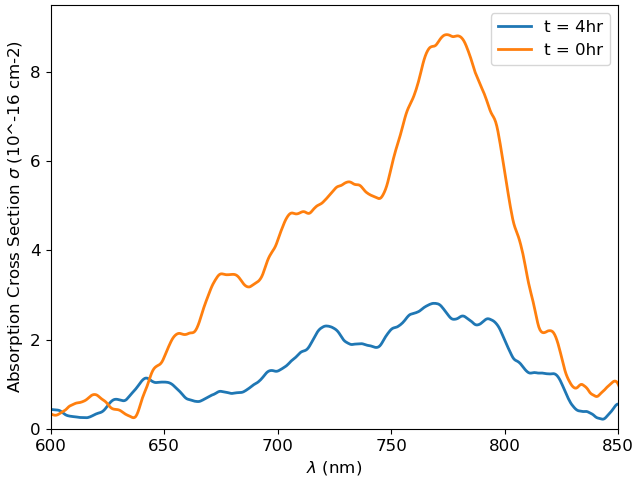
\includegraphics[width=0.6\textwidth]{./Figures/ICG/abc_time.png}
	\caption{Degradation of a 4.5ppm initial concentration sample after 4hrs of light exposure reduced to a 2ppm concentration.}
	\label{fig:icgphoto}
\end{figure}
\clearpage


\subsubsection{ Fluorescence}
Photoluminescence in the dye is emitted in the range of 750-900nm. overlapping with the absorption spectrum. The peak emission wavelength for ICG varies within 800nm-820nm\cite{philip, saxena} when excited at 780nm and decreases as solution concentration increases, The dimmerization effects are attributed to (a) The formation of weakly fluorescent ICG molecular aggregates at high concentrations (b) self-quenching and (c) re-absorption of the emitted fluorescence by the ICG molecules due to overlap of the absorption and emission spectra. In the J-aggregate form  the excitation wavelength shifts to 834nm and the emission peak at 890nm, however, low quantum yield and strong light scattering does not lend to accurate measurements\cite{rotermund}.  
\begin{figure}[!htb]
	\centering
	\foreach \x in {wl_fluor, wl_fluor_absp}
	{ 
		\begin{subfigure}[b]{0.47\textwidth}
			\includegraphics[width=\textwidth]{./Figures/ICG/\x.png}
			\caption{}
		\end{subfigure}
	}
	\caption{(a)Fluoresce spectrum of 4.5ppm sample (b) Maximum fluorescence and maximum absorption spectrum of 4.5ppm initial concentration sample}
	\label{fig:icg_spec}
\end{figure}
\clearpage

